\begin{refsection}


\chapter{Modeling ion thermal transport in the RFP}\label{ch:physics}

% I think you should mention that prior work on understanding on ion heating and heat transport has concentrated on understanding the mechanisms of rapid magnetic reconnection leading to rapid anomalous ion heating while also leading to rapid transport of electron heat. Cite:    % * Chapman PPCF 52, 124048 (2010)
% * Gangadhara S, Craig D, Ennis D A, Den Hartog D J, Fiksel G
%     and Prager S C 2007 Phys. Rev. Lett. 98 075001
% * Gangadhara S, Craig D, Ennis D A, Den Hartog D J, Fiksel G 
%     and Prager S C 2008 Phys. Plasmas 15 056121
% What's new here is that you are considering the ion heat transport under quiescent conditions in the best performing MST plasmas and that even in the absence of strong, rapid reconnection events there are heating mechanisms still present, particularly in the edge of the plasma. Then cite   
%---
%Added. -X

A full understanding of the broad topic of ion thermal transport is difficult to tackle. Past efforts to understand transport in MST have concentrated on the sawtooth crash and it's effects on transport. The magnetic reconnection of the sawtooth events leads to rapid and anomalous ion heating as well as rapid heat loss from electrons\cite{Chapman2010}, and the ion heating response to several sub-catagories of magnetic reconnection has also been studied\cite{Gangadhara2008}. For this work, I focuses instead on the ion thermal transport behavior during quiescent conditions in the absence of strong and distinctive reconnection events, through residual turbulence is still present. This quiescent plasma conditon is achieved through PPCD. Unlike improved confinement through the Quasi-Helical State (QSH), PPCD plasmas are highly axisymmetric and have reduced stochasticity, making them ideal for a simplified 1-D model. Previous work has established preliminary 0-D and 0.5-D power balance calculations for the ions\cite{Waksman2013} which are limited in usefulness as they cannot distinguish the likely differences that exist between the core and the edge/gradient region. A 1-D model is the logical next step in the investigation of ion heat transport and anomalous heating. This chapter aims to examine the ion thermal transport physics included in the model and a justification for excluding other transport mechanisms.  I will briefly review thermal equlibration between electron and ions, as well as classical collisional thermal diffusion. Then I will discuss the effects of neutral particles and the particle flow on transport. The proper treatment of neutrals turns out to be quite important in PPCD. Charge exchange neutrals are not confined by magnetic fields and have a long mean-free-path giving them a significant influence on a per reaction basis. This is followed by a discussion of neoclassical and stochastic effects on heat transport and why they are not modeled by the code. At the same time, I aim to distinguish their effects on particle transport vs. on thermal transport, and how they are ultimately treated in the final comparison with data. 

%Note that this chapter introduces a large number of variables and it is not always practical to note their meaning with every equation. Please refer to appendix \ref{app:term} for notes on notation and terminology. 

\section{Modeled ion transport mechanisms}
This model attempts to include well understood heating terms that are known to be active. In this section, I explore the known heat transport mechanisms being modeled and their general physics basis and characteristics. Some of these mechanisms also couple with particle density change, which may result in the phenomenon where the power is positive (ie, ion thermal energy increasing) but the ion temperature is decreasing. This is discussed in more detail in appendix \ref{app:term}

\subsection{Electron ion equilibration}\label{sec:equilibration_power}

In a plasma where the temperature is different between two species, Coulomb collisions cause a transfer of thermal energy from the hotter to the colder species. This is thermal equilibration. In PPCD plasmas, the electron confinement is significantly improved compared to standard RFP plasmas and $T_e$ rises significantly compared with the pre-PPCD period to levels significantly above $T_i$. Thus, equilibration is a heating term for the ions. This is a reflection of the fact that MST plasmas are primarily heated ohmically, which is nearly entirely an electron heating mechanism. Particularly in PPCD plasmas, where anomalous heating mechanisms available to ions are reduced, the thermal equalization becomes important. The equalibration power can be calculated as\cite{Braginskii1965}:
\begin{equation}
    P_{\text{eq}} = \frac{3}{2}n_i\nu^{i/e}(T_e - T_i)
\end{equation}
where $\nu^{i/e}$ is the thermal equilibration frequency, defined as\cite{Greene1973}:
\begin{equation}
    \nu^{i/e} = 5.69\times10^{-27}\frac{(m_e m_i)^{1/2}(Z_e Z_i)^{2} n_e ln \Lambda}{(m_iT_e + m_eT_i)^{3/2}}
\end{equation}
% Make sure to indicate where this forumlation for the energy equilibration frequency comes from. The NRL formulary is NOT a primary source. This is probably from Braginskii's collisional transport paper, but you should check your references.
% Added the sources. --Xing
It is important to note that $\nu^{i/e}$ is not the Lorentz collision frequency but is related to the energy relaxation frequency. Due to the mass discrepancy between ions and electrons, energy transfer between the two is small per collision. Thus, the calculated equilibration heating from even the lower temperature edge region is relatively small even though the Lorentz collision frequency is relatively fast. This poor coupling helps explain why in PPCD plasmas $T_e$ can significantly exceed $T_i$. A typical profile is shown in Fig.~\ref{fig:P_eq}.

\begin{figure}[!htb]
	\centering
	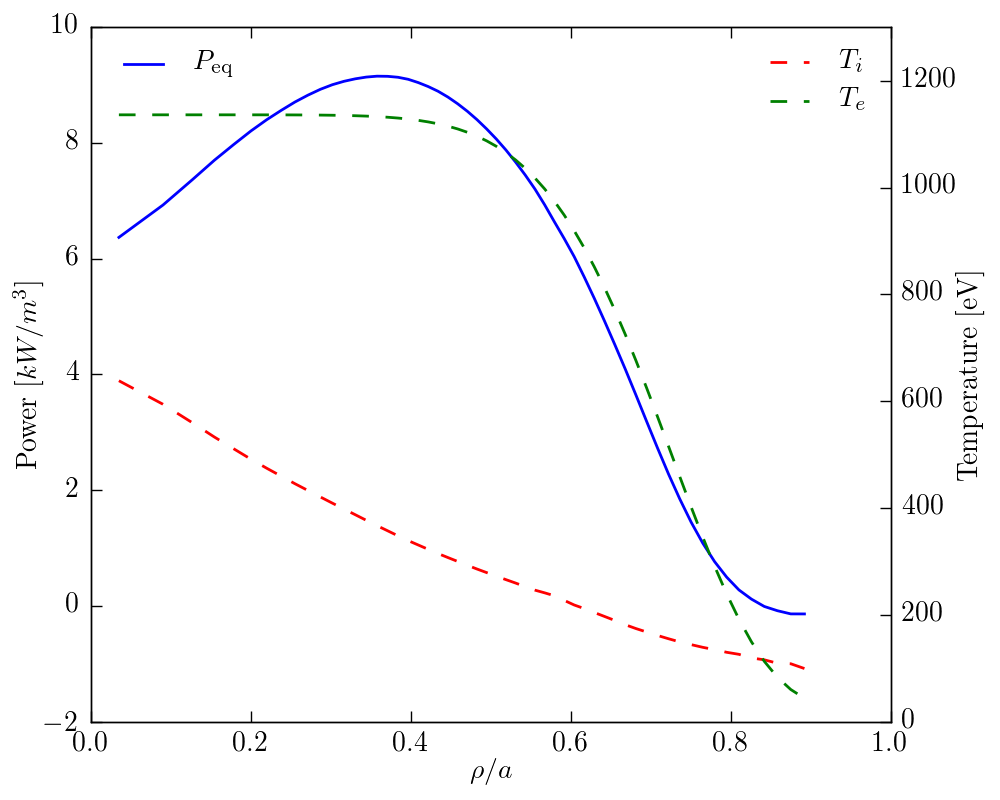
\includegraphics[width = 0.75\linewidth]{./transport_modeling/p_eq.png}
    \caption[Example equilibration power profile.]{An example of equilibration power profile in PPCD plasma conditions. The plot also show the $T_e$ and $T_i$ that forms the basis of this calculation.}\label{fig:P_eq}
\end{figure}%
%%% MAKE SURE TO EXPLAIN WHAT EACH CURVE MEANS IN THE CAPTION. P_Cond means equilibration power? --- MDN
%Corrected label on plot, and clarified the caption somewhat. --Xing


%\begin{figure}[!htb]
%	\centering
%	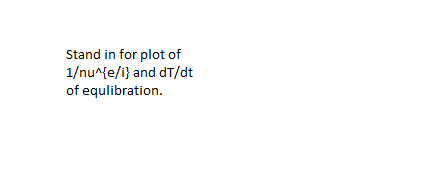
\includegraphics[width = 0.75\linewidth]{./transport_modeling/tau_eq.png}
%    \caption[Electron ion thermal equlibration time]{An example of equlibration profile in PPCD plasma conditions. The plot also show the $T_e$ and $T_i$ that forms the basis of this calculation.}\label{fig:tau_eq}
%\end{figure}%

This heating term would increase as the PPCD period progresses due to the increase in $T_e$ and the relative constancy of $T_i$ significantly increasing the temperature differential. However, the increase in heating is smaller than what might be expected at first sight as the increase in temperature decreases the collisionality. This may indicate that Ohmic heating is not efficient for ion heating, however, higher densities expected in future devices is expected to mitigate this concern. 
% Looking at Eqns. 2.1 and 2.2, I would expect the equilibration power to drop with electron temperature since P_ei is roughly proportional to Te / Te^{3/2} ~ Te^{-1/2} when we neglect the small contribution from T_i in the denominator which is weaker by the electron/ion mass ratio.

%Clarified. It is due to the fact that T_i is effectively staying constant, therefor (T_e-T_i) is growing quickly. --Xing

\subsection{Classical thermal conduction}\label{sec:thermal_cond}

Classical thermal conduction refers to the heat diffusion due to Coulomb collisions. Note that this is not the same as the particle transport and the thermal energy associated with that movement. In an cartoonish approximation, thermal diffusion is caused by a hotter ion colliding with a colder ion on an adjacent field line during their gyro-orbits. Energy is exchanged when the two particles are exchanged while momentum is conserved and thus no net particle flow results. Unlike the particle diffusion, the thermal conduction is related to like-particle collisions, and depends on the tmer. The thermal conduction is thus dependent on the temperature gradient and can be calculated as\cite{Shafranov1966}:
\begin{align}
    P_{\text{cond}} &= \nabla\cdot\vec{q}_{\text{cond}} \\
    &= \frac{1}{\rho}\frac{\partial}{\partial\rho}(\rho\kappa_{\perp}\nabla T_{i})\\
    \kappa_{\perp} &= \frac{2n_ikT_i\nu_i}{m_i\omega_{ci}^2}
\end{align}
where $nu_i$ is the ion-ion collision frequency.
% You need to specify what \nu_i is here. I believe this is the ion-ion collision frequency.
%---
% Added -Xing

In comparison with the other terms in the ion power balance, the thermal conduction term is relatively small. It is, however, simple to calculate and still included in the model. A typical $P_{\text{cond}}$ profile is presented below. In terms of power density, it is most 'active' in the core where the density is high, and gradient is still significant (note that the radial gradient have a $\frac{1}{\rho}$ factor inside the derivative). In the edge the particle density have decreased to a level where the power density from conduction is low despite the high gradient.
% From the figure you include, it looks more like the conduction term is weak in the edge (fluctuating around 0) and on the order of a couple kW/m^3 in the core. I assume the negative value implies outward transport.
%---
%Reworked after investigating further. -X

\begin{figure}[!htb]
	\centering
	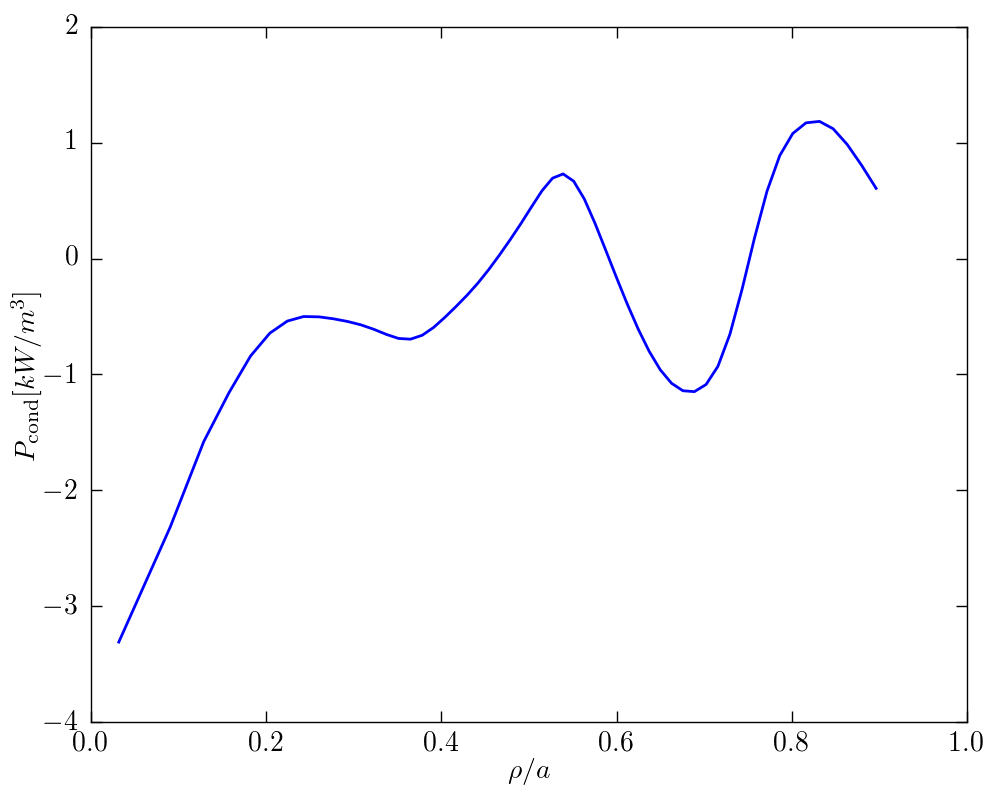
\includegraphics[width = 0.75\linewidth]{./transport_modeling/p_cond.png}
    \caption[Thermal conduction profile]{An example of thermal conduction profile. Note the axis, this term is significantly below the equilibration term presented above, and most of the terms that I'll present later.}
    \label{fig:p_cond}
\end{figure}%

\subsection{Charge exchange and neutral transport}\label{sec:neutral_physics}

MST's thermal transport is significantly affected by the neutral population through charge exchange. Charge exchange is the process where a neutral particle, typically atomic deuterium for MST, 'gives' it's electron to an ion due to a collision. Since only the electron mass is exchanged in the collision, there is approximately no momentum exchange in the collision.
This causes the hot ion to become neutral and thus un-confined. Although the neutral fraction of the plasma is very low, charge exchange can have an out-sized effect due to the neutral essential 'by-passing' the entire magnetic confinement concept. 
% The out-sized effect has more to do with the mean-free-path of the neutral generated by charge exchange. Normally, the neutrals have an energy of a couple eV due to the dissociation energy of the molecule. Neutrals that are generated by charge exchange with thermal ions result in fast neutrals with energies exceeding 10 eV. At the resulting velocity, the neutral travels a significant distance (greater than an ion gyroradius) before experiencing an ionizing collision from a thermal electron. This makes it a relevant transport mechanism.
This is especially significant in improved confinement (PPCD) plasmas where other mechanisms are reduced. The charge exchange loss can be calculated as:
\begin{align}
    P_{\text{CX loss}} = n_0 n_i <\sigma v>_\text{CX} (T_i - T_0)
\end{align}
where $T_i$ is the ion temperature, $T_{0}$ is the neutral temperature.

In previous estimates, the neutral fluid is assumed to be cold \textit{i.e} $T_0 = 0$. However,the mean free path of a "cold" neutral is very short (<1cm), but edge neutrals may undergo subsequent charge exchange collisions resulting in higher temperature neutrals that can penetrate into the plasma. Consequently, neutrals in the core are mostly generated near the mid-radius and have a temperature comparable to mid-radius ions. At the same time, a charge exchange neutral created from thermal neutral in the core, if traveling through core-like conditions, has a mean free path
shorter than the minor radius, implying a fraction of such neutrals would undergo secondary ionization or additional charge exchange reactions. 

\begin{figure}[!htb]
	\centering
	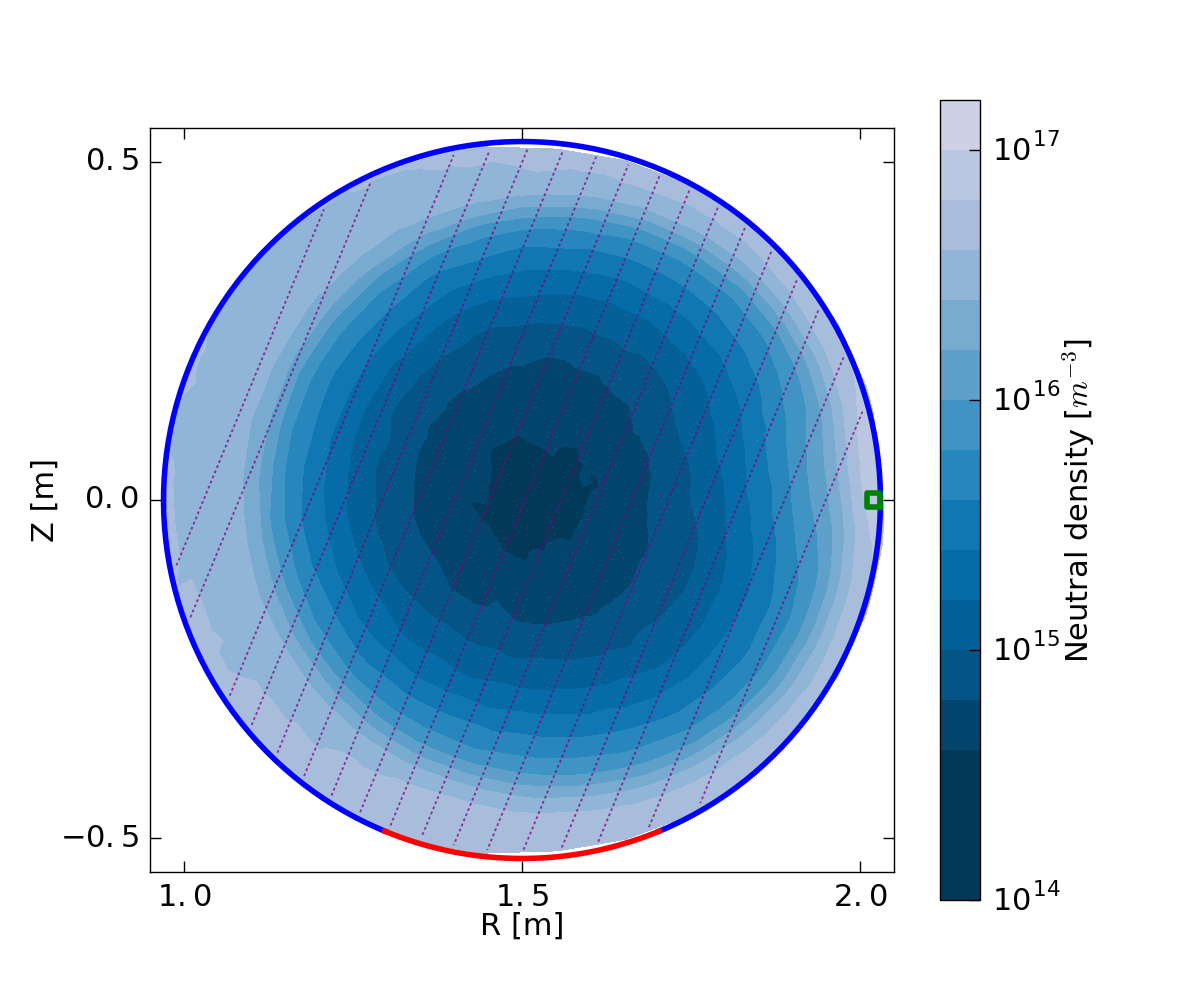
\includegraphics{./transport_modeling/neutral_n.png}
    \label{fig:n_n_0}
    \caption[Typical neutral density profile]{A typical neutral density has nearly 3 orders of magnitude drop between edge and core densities. This makes the determination of the core density difficult without modeling efforts. The analysis that produced this density profile are explained in more detail in section \ref{sec:neutral_results}}
\end{figure}%

As far as terminology and conceptualization is concerned, the charge exchange 'transport' is presented as two terms in the modeling. The first is the charge exchange loss term itself $P_{\text{CX loss}}$, in which when an charge exchange reaction occurs, the difference in energy is considered lost from the ion fluid immediately. This lost energy is not entirely lost, but instead should be thought of as part of the neutral fluid's thermal energy. This thermal energy exchange reduces $P_{\text{CX loss}}$ by reducing the temperature difference between the ion and the neutral fluid. If the fast neutrals generated by this process undergo subsequent electron impact ionization, then this thermal energy will return to the ion fluid. This process is marked as a separate term noted as $P_{\text{e-imp}}$. It is important to note that while the electron impact brings the thermal energy 'back' to the ion fluid, it does not (typically) cause heating as the process is also a particle source term that (typically) is adding cooler ions to the fluid. In this work, the net power density from these processes are noted by $P_{\text{CX}}$ for simplicity. The consequences of mechanisms that contribute both particle and heat are discussed more directly in Appendix \ref{app_sec:power_terms}.

From a diagnostic point of view, the neutral density is not a straight forward quantity to measure. The neutral density drops precipitously towards the core of the plasma where the temperature is high. Measurements of neutral emissions, in MST's case the deuterium Balmer-alpha line emission, only reflects the edge neutral density as that's where the emission is coming from. The emission from the core is so low such that it is buried in the noise and fluctuations of the edge emission. Therefore, physics-based equilibrium modeling is needed to construct self-consistent core neutral profiles that produce the observed $D_{\alpha}$ emissions. Temperature would be even more difficult to measure as it's not accessible with typical spectroscopic methods. Recently on the HIT-SI3 experiment, researchers have been able to use a two-photon Laser Induced Florescence diagnostic to directly measure the density and temperature of deuterium neutrals\cite{Elliott2016}. However, such a diagnostic is not available for MST and would likely be unable to measure the low neutral density expected in MST's core. 

Instead, Monte Carlo modeling is used to solve the issues detailed above. Monte Carlo modeling uses representative particles sampled from a distribution. Their location and velocity is tracked and relevant physical interactions and reactions are simulated with appropriate physics-based probability distributions. This process is then repeated until the parent population is thoroughly sampled. The 'fate' of any given sample is not particularly illustrative, but the collective results of all of the samples result in a distribution (or total) of the quantities of interest. For this work, the particular quantity of interest is not only the neutral density and temperature, but also the two power terms described above ($P_{\text{CX}}$ and $P_{\text{e-imp}}$) which are tallied through the simulation directly. The simulation code used to achieved this is DEGAS2 developed at PPPL\cite{Stotler}, and the details of it's implementation as part of the model are detailed in section \ref{sec:DEGAS2}. The result from the neutral simulation regarding the charge exchange loss and electron impact ionization is complex and will be presented more fully in section \ref{sec:neutral_results} after the implementation of DEGAS2 have been described. 

\subsection{Particle flow, compression, and decompression}\label{sec:flow_effects}

When the ion fluid moves, it carries its thermal energy with it. 
% This statement is not accurate. A single particle doesn't have thermal energy, only it's own kinetic energy. When we talk about thermal energy we are referring to a population of particles. It would be good to go through your description of Monte Carlo simulation and rewrite it so that you refer to a parcel of fluid (indicating a population of particles in thermal equilibrium). The Monte Carlo simulation tries to represent the dynamics fluid parcels by tracking the trajectories of sample particles from the fluid parcel.
%---
%Reworded above statement. I'm entirely clear about your comment on the Monte-Carlo descriptions though. I edited the wording to be clearer and better reflect the wording in DEGAS2 manual. let me know if you still find it problematic. -X
In this section I will speak generally regarding flow, but in the modeling work only the radial flow are considered as the symmetry assumptions implies no meaningful effects from toroidal and poloidal flow. The particle continuity equation can be written as:
\begin{align}
    \partialt n + S_{\text{tot}} = -\nabla\cdot(n\vec{V}) \label{eqn:continuity}
\end{align}
where $S_{\text{tot}}$ is the total source term. Extending the continuity equation to the thermal energy carried by the particles, and ignore the source term by focusing on the effect of the particle flow, we get:
\begin{align}\label{eqn:thermal_continuity}
    \partialt nT = -\nabla\cdot(nT\vec{V})
\end{align}
In an compressible fluid, however, there is the potential of compression work by external sources, so the equation becomes:
\begin{align}
    \frac{3}{2}\partialt nT &= -\frac{3}{2}\nabla\cdot(nT\vec{V}) - nT\nabla\cdot\vec{V}\\
    &= P_{\text{flow}}\nonumber
\end{align}
where the the first term on the righthand side is the \emph{flow conservation} term and the second term is the \emph{compressional work} term. For convenience of reference in the rest of this work, we define $P_{\text{comp work}} \equiv - nT\nabla\cdot\vec{V} $, and $P_{\text{flow cons}} \equiv -\frac{3}{2}\nabla\cdot(nT\vec{V})$.


\subsubsection{A discussion on which velocity is proper in calculation thermodynamic compressional work}

The compressional work term needs a more detailed examination from the fact that not all net decompression would invoke the work term. This makes it important the 'correct' velocity is used to calculate the work term. To begin, consider the difference between adiabatic expansion and Joule free expansion. In adiabatic expansion, a gas in a fully insulated chamber expands against a 'piston' and does work on it. The net power on the gas is thus $P_{\text{work}} = - PdV$ where $P$ is pressure and $V$ is volume. Joule free expansion involves two adjacent chambers, one of which is filled with a gas with finite temperature and pressure, and the other is in perfect vacuum. The two chambers are perfectly insulated. At a $t=0$ the wall between the two chambers is broken and gas from the first chamber is allowed to flow to the second until the pressure equilibrates. In this process, the expansion does no work and no net energy is lost; it merely moved to be spread over a larger space. 

To examine the implications for a plasma, we start with a thought experiment. Imagine a slab plasma adjacent to a perfect vacuum confined by a static magnetic field at equilibrium. The plasma has finite temperature with no transport mechanisms active except for what is about to be specified. The plasma is not perfectly confined, and a small flux of particles is being lost to the vacuum. In this situation, the only energy lost is that carried by the particle flux, without a work term. As a result, the temperature (energy per particle) of this plasma would not change. If the $- nT\nabla\cdot\vec{V}$ work term was to be applied in this situation, then the temperature of the remaining plasma would cool, which would conflict with the understanding of the microscopic mechanics of the plasma. This situation would be analogous to the Joules free expansion mentioned above, with the 'wall' in the joules free expansion case replaced with an imperfectly confining magnetic field. By a similar analogy, plasma compression via the movement of a perfectly confining magnetic flux surface can be compared to a compressing piston. It's useful to note that there is no free compression. If compression occurs, then \emph{something} has done work, and it's a matter of finding what. This is also why free expansion is considered an irreversible process, as there is no equivalent reversing process.

In real PPCD plasmas, however, these two mechanisms are not so easily separated. During the early phase of PPCD, the reversal surface is observed to move inwards, as does the $n_e$ gradient region. As will be discussed in section \ref{sec:eb_pinch}, there is an inward pinch likely related to an $\vec{E}\times\vec{B}$ drift. However, in the outer half of the plasma the net particle flow is outwards across flux surfaces due to particle transport mechanisms outside of the consideration of this thesis. This, in the thermodynamic analogy, would be akin to a leaky piston moving inwards, but the net particle velocity being outwards. The velocity use to calculate $P_{\text{flow cons}}$ should be the net velocity, as the the ions will carry their energy with them whatever the 'reason' of their movement. However, the velocity used in the work term should be the velocity associated with the mechanism by which the work is done. In this case, the \ecb drift and the movement of the flux surface associated. The implementation and consequences of this, as well as the determination of the \ecb flux and it's association with compression is discussed in much more detail in section \ref{sec:eb_pinch}.

\section{Unmodeled terms and mechanisms}

\subsection{Neoclassical effects}\label{sec:neoclassical_cond}

Neoclassical effects are, in approximation, those that arises due to the toriodal nature of the magnetic confinement devices. In short, due to the nature of Ampere's law, $B_t$ on the inboard side is higher than the low field side, and drops as $~1/R$. This fact is important enough in the Tokamak that the inboard side is typically referred to as the high-field side, and the outboard side as the low-field side. As a given field-line travels poloidally around the plasma volume, particles see varying $|\vec{B}|$ and effectively experiences a magnetic mirror. The slower particle with insufficient parallel momentum to complete a full poloidal orbit are referred to as trapped. They are reflected by the mirror effect and 'bounce' in the opposite poloidal direction. But $\nabla B$ and curvature drifts give the poloidal path of the particle a certain width, giving it a crescent shape. This trajectory is called the banana orbit, and the width the banana width. For the Tokamak geometry, the existence of the banana orbit enhances the collisional transport experienced in low collisionality regimes since a collision may move a particle a banana width from it's previous orbit average location instead of a gyro-radius. This effect is less important as the collisionality increases since the particles are no longer able to complete banana orbits before collisions alter their path. Further, the collisional transport is typically not \emph{directly} effected by neoclassical considerations. While the banana width is larger than the gyro-radius in Tokamak geometry, that is not typically the case for RFPs including the MST. The text book calculations of banana width and neoclassical transport is (typically) made with Tokamak approximation that $B \approx B_t$ which is not valid in the RFP. The proper calculation in the RFP geometry is significantly more complex. It was performed by Oshiyama and Masamune \cite{Oshiyama1983} who found that the neoclassical enhancement of transport was small in axis symmetric RFP geometry. Neoclassical transport in the RFP was again studied via Monte Carlo methods by Chen \textit{et al.} \cite{Chen1992}, and it was found that the neoclassical transport due to guiding center drift was negligible, where was indirect effects such as turbulence from particle trapping can have a significant effect on transport. With this in mind, the neoclassical conduction is ignored in the ion thermal transport model.
%This section edited and updated as per our email discussion. -X

\begin{figure}[!htb]
	\centering
	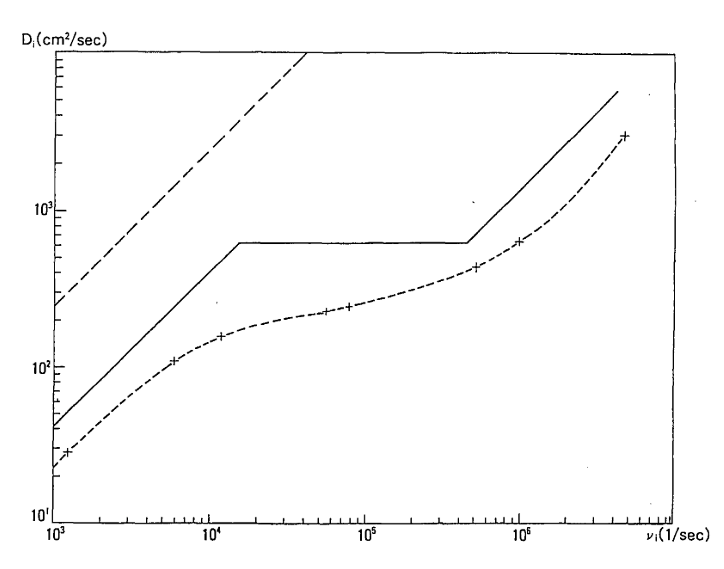
\includegraphics[width = 0.75\linewidth]{./transport_modeling/neo_class_diff.png}
    \caption[Neoclassical diffusion coefficient for RFPs]{Neoclassical diffusion coefficients vs collision frequency. The dashed line is the classical diffusion, the solid is from analytical calculations in RFP geometry, and the dotted with crosses line is of the Monte Carlo results of neoclassical diffusion. (Reproduced from Chen \textit{et al.}\cite{Chen1992})}
\end{figure}%

The trapped particle population will also affect the plasma stability, turbulence, and, indirectly, the transport properties. For example, the neoclassical correction to the Spitzer resistivity is important for the electron thermal transport, and trapped-electron mode turbulence is also known and measured for PPCD plasmas. These are not with in the scope of this thesis. However, they are not so much ignored but incorporated indirectly. The electron temperature is measured and used as an input to the model, so it effectively accounts all electron physics at or slower than the cadence of measurement. The effect of any induced particle transport is indirectly incorporated through the particle continuity equation, and the determination of net particle flux, discussed in section \ref{sec:eb_pinch}

\subsection{Stochastic effects}\label{sec:stochastic_effects}
No discussion of transport in the RFP is complete without a discussion of the effects of stochasticity. However, the full effects of stochasticity is not known to an analytically extent. In their well known paper, Rechester and Rosenbluth\cite{Rechester1978} detailed a way to compute thermal diffusion due to stochasticity. An estimate of the stochastic thermal conduction can be made by extending done by Anderson \textit{et al.}\cite{Anderson2005} on electrons. For stochastic conduction, $\chi \propto v_{\text{th}}$, and assume $T_e = T_i$, then $\chi_i = \sqrt{\frac{m_e}{m_i}}\chi_e$. Taking the stochastic $\chi_e$ calculated for PPCD by Anderson, and using above estimations, a reference value for stochastic conduction is arrived at (see figure \ref{fig:p_st}), and found to be similar to classical conduction, which itself is small compared to other power terms. In PPCD plasmas, $T_i$ is smaller than $T_e$ ($\frac{T_i}{T_e} \approx 0.3-0.6$ except the very edge), which would further reduced $\chi_i$ with respect to $\chi_e$ and reduced the estimate. 
\begin{figure}[!htb]
	\centering
	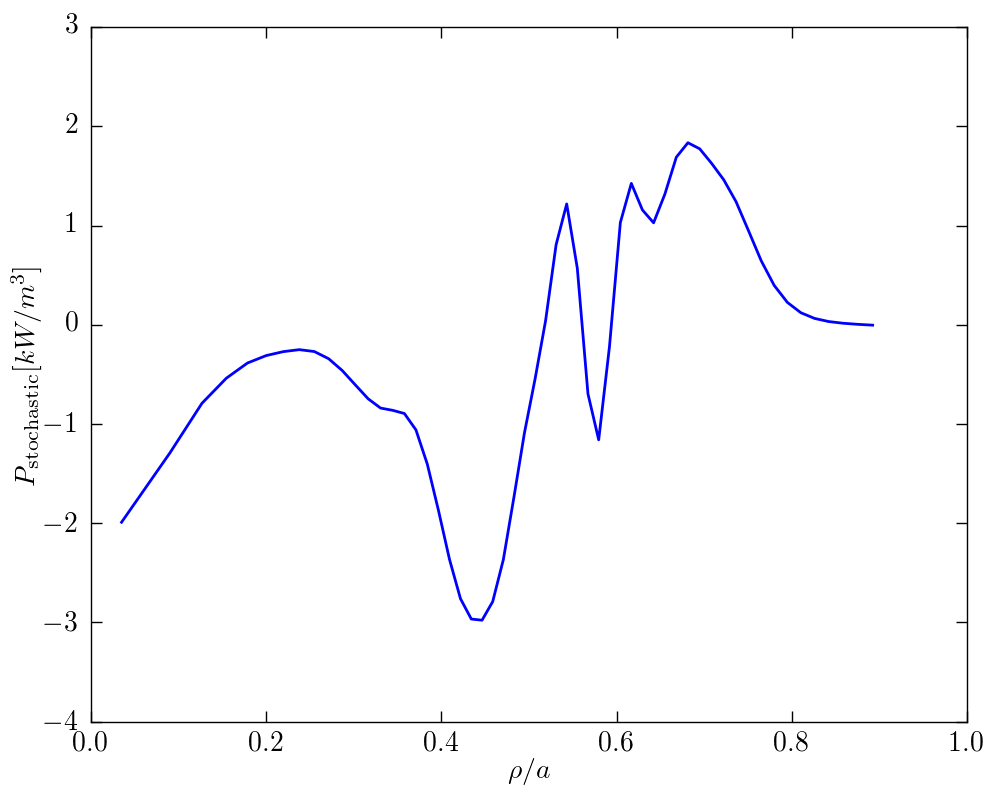
\includegraphics[width = 0.75\linewidth]{./transport_modeling/p_st.png}
    \caption[Estimation of stochastic conduction]{Estimation of stochastic conduction by extending previous work done on stochastic conduction of electrons by Anderson \textit{et al.}\cite{Anderson2005}.}
    \label{fig:p_st}
\end{figure}%

However, the actual stochastic transport is complex and can yield unexpected results. To more accurately understand the effect of stochasticity, thesis-es worth of complex simulation modeling work needs to be done. Further, stochasticity is not static, but inextricably linked with fluctuations and turbulence. In the case of ions, stochasticity is proposed as a heating mechanism associated with sawtooth events\cite{Fiksel2009}. Being that stochasticity is both reduced in the PPCD plasma, and that it is likely associate with the anomalous heating that I aim to isolate and investigate, I take the approach of categorizing the stochastic effects on heat transport as a part of the anomalous heating. A quantification and localization of the anomalous heating is instructive in the discussion and investigation into stochastic mechanisms, and this will be discussed in more detail in section \ref{sec:anomalous_heating}. It is important to note that similar to neoclassical effects on particle transport, the stochastic effects on \emph{particle transport} is indirectly included via the continuity equation, as the density observations are treated as an input parameter. Whereas the stochastic effects on \emph{thermal transport} is treated as anomalous.


% I think that you could provide an estimate of how large you may expect the stochastic transport to be in these plasmas. Biewer et al., PRL 91, 045004 (2003) shows how to calculate the Rechester and Rosenbluth thermal conductivity for the electrons and Anderson et al. Phys. Plasmas 12, 056118 (2005) shows values of the electron stochastic heat transport for PPCD plasmas. The only difference between the two formulations is that the ions travel at a much lower thermal speed than the electrons so the equivalent thermal conductivity will be down by the ratio of the ion thermal speed to the electron thermal speed. In Anderson (2005), Fig. 5 he shows that the measured electron heat conductivity is ~ 10 m^2/s. The equivalent stochastic ion heat transport will be down by roughly the square root of the mass ratio due to the ratio of the thermal speeds, so I estimate that the ion stochastic heat conductivity will be ~ (10 m^2/s) (9.11E-31 kg / (2*1.67E-27 kg))^0.5 ~ 0.2 m^2/s.
%
% I think that if you calculate the ion heat transport due to this term, you'll get something on the order of a couple kW/m^3 just like the collisional heat conduction term. So according to your ordering, you should neglect both processes.

%---
%added estimate. -Xing



\section{Summary of ion thermal transport in the RFP}\label{sec:transport_summary}

In this chapter I have laid out the ion thermal transport physics incorporated into the model. Starting with the simple, classical thermal equlibration between electron and ions, and the classical collisional thermal diffusion, both of which are well known and easy to calculate. The transport effects of the neutral fluid and particle flows are more complex, and as you will see, forms a significant part of the work of this thesis. The proper treatment of the neutrals and especially the fact that they have a temperature is important to quantifying their effects, and in the result section I will demonstrate that heat transport due to $P_{CX}$ can exhibit behaviors that are not intuitive, especially within the $Q = -n\chi\nabla T$ framework where one seeks to quantify transport with a calculated $\chi$ value. 

A numerical model is built to predict 1-D ion temperature profile by calculating these terms. The model implementation will be discussed in detail in the next chapter, along with the diagnostics used. However, at it's core, the model numerically integrates the following differential equation,
\begin{align}
    \partialt E_\text{thermal} = P_\text{e-i} + P_\text{cond} + P_\text{CX} + P_\text{flow} + P_\textit{ad hoc}
\end{align}
In the simplest form, the model is a numerical integration of this equation in time, arriving at temperature predictions. The various terms are integrated and calculated at each step with the appropriate diagnostic input and equilibrium reconstruction. The end goal is a comparison of the model prediction with measurement of $T_i$ provided via CHERS. Having explored the physics being modeling in this chapter, I will go into details about the implementation in the next.  


\printbibliography%[title={Section bibliography}]
\end{refsection}

